\chapter{Лысая гора на левом берегу}
   
Многие люди и не знают, что она была тут, а некоторые не ведают, что сохранилась и поныне, но застроена и перерыта. При слове «гора» в разуме возникает нечто большое, хорошо заметное издалека. Однако проезжая, скажем, в вагоне метро и глядя через окно на левый берег, ничего подобного не замечаете. Всё плоско!

Когда же вы ходите по местности своими ногами или вкручиваете педали на велике, то представление о левом берегу как о плоском оказывается весьма ошибочным. Горы есть, просто большей частью они плавные, не столь крутые, как правобережные. Горы-дюны.

Лысая гора тянулась чередой таких песчаных дюн от северной части озера Святище (у Никольской слободки) на север, заходя за восточную часть Воскресенской слободки.

Впрочем, уже в 19 веке южная граница горы как урочища сместилась на север от Броварского шоссе, ибо к Святищу подобралось жильё. Однако на моем любимом генплане Киева 1750 года Лысой горой подписан северо-восточный берег Святища, поэтому предполагаю, что тогда за Лысую гору понимали самую южную часть «хребта». Но в 19 веке это представление связывалось с дюнами уже по другую сторону Никольской слободки – на северо-запад от станции метро «Левобережная».

Какие же части Лысой горы уцелели по 2016 год? Сейчас сложно быть точным из-за изменений местности. Давайте почитаем сначала, что писали о ней краеведы 19 столетия.

В книге 1864 года Николая Сементовского «Киев, его святыня, древности, достопамятности и сведения необходимыя для его почитателей и путешественников» находим:

\begin{quotation}
Левый берег Днепра, т.е. малороссийский, против г. Киева, совершенно отлогий. Он покрыт трехверстными в ширину поемными лугами, за коими разбросаны селения, а за ними тянутся по местам сосновые леса. За приднепровскими лугами, на левом берегу Днепра\footnote{Точнее, Черторыи, но ежели ее полагать рукавом Днепра, то выходит и Днепра. Днепр тогда был соединен с Черторыей проливом Пробитцем.}, между слободами Никольскою и Воскресенскою виднеется песчаная небольшая возвышенность, это преслоутая Киевская Лысая гора, которая некогда составляла берег Днепра. Киевския ведьмы и Лысая гора, на которую оне, по преданию ведущемуся, из глубокой древности слетались на шабаш, известны по сказкам и легендам не только в пределах России, но и во всем славянском мире.
\end{quotation}

В книге «Киев теперь и прежде» М. М. Захарченко, 1888 года, сказано:

\begin{quotation}
За лугами, против Киева, виднеются две слободки, Никольская и Воскресенская, а между ними одиноко стоит среди равнины, покрытой лесом, небольшая песчаная возвышенность, известная в южно-русских преданиях под именем Лысой горы (и дана ссылка на книгу Сементовского. – Киев, стр. 6. Киев 1881 г.).
\end{quotation}

П. Полевой во втором томе «Очерки русской истории в памятниках быта» (1880, С-Петербург, 1880, стр. 4) пишет:

\begin{quotation}
За при-днепровскими лугами, между слободами Никольскою и Воскресенскою, одиноко возвышается среди равнины прославленная в южно-русских преданиях Лысая гора.
\end{quotation}

Закревский в первом томе «Описания Киева» сообщает:

\begin{quotation}
По соседству Черторыи с Лысою горою, можно догадываться о происхождении ея названия.
\end{quotation}

В первом томе же «Описания Киева», в параграфе 81, Закревский пишет:

\begin{quotation}
Горя сия находится с левой стороны Днепра, в виду Киева. Начинаясь вблизи шоссе от Цепнаго Моста\footnote{Современное Броварское шоссе.}, она простирается, мимо селения Воскресенскаго, небольшим песчаным возвышением почти на четыре версты до села Вигуровщины.
\end{quotation}

В книге «Спутник по г. Киеву. Иллюстрированный путеводитель по Киеву и его окрестностям. Издание VII-е С. М. Богуславского» (Киев, 1912 год) сказано:

\begin{quotation}
Лысая гора, – знаменитое место  сборища киевских ведьм, – возвышается длинным песчаным холмом на левом берегу Днепра, в пределах Черниговской губернии. Возвышенность эта начинается близ Николаевского цепного моста и тянется версты на четыре до села Вигуровщины. Из города она вырисовывается довольно явственно с верхней площадки памятника св. Владимиру. 

Это и есть настоящая, воспетая народной фантазией «Лысая гора», где местныя, иногороднии, и даже чужестранныя ведьмы, согласно поверью, собираются, чтобы отпраздновать свои шабаши. 

Кроме этой подлинной Лысой горы, в пределах Киева существует еще несколько возвышенностей, известных под тем же названием и пользующихся столь же нелестной репутацией. Одна из них лежит на Печерске близ саперных лагерей, дав название одному из крепостных фортов («Лысогорский форт»), другая расположена за оградой Михайловского монастыря, с северо-восточной стороны; это последнее место называлось когда-то чертовым беремищем. Лысогорский форт получил в последнее время печальную известность как место совершения казней над осужденными по приговорам военно-окружного суда.
\end{quotation}


На север от Левобережки, в сторону Воскресенки – железная дорога и станция Киев-Днепровский. За нею – Деснянская водопроводная станция на длинном возвышении. По карте РККА 1930-х годов там видна дикая бугристая местность со странно ровной линией восточного склона.

Проспект Освободителей проложен вдоль Лысой горы, а следующая за ним к северу основная магистраль Воскресенки – бульвар Перова – вдоль горы и по ней. 

Раньше, до строительства жилых кварталов, этой дороги не было. Существовала дорога, где ныне проспект Освободителей, и отходящая от него Воскресенская улица (идущая к жилмассиву Воскресенскому).

А там, где Перова, на отрезке от проспекта Освободителей до широты дома номер 14, в первой половине 20 века был хвойный лес, и севернее шли уже пески по дюнам, в том числе Лысой горы. Воскресенская же слободка лежала к востоку от бульвара Перова, между ним и озером Радункой, на севере ограничиваясь нынешней улице Кибальчича. Сейчас тот район считается жилмассивом Радужным, а Воскресенкой – район на восток от Перова, где в 20 веке было пусто, песчаные дюны.
\vspace*{\fill}
\begin{center}
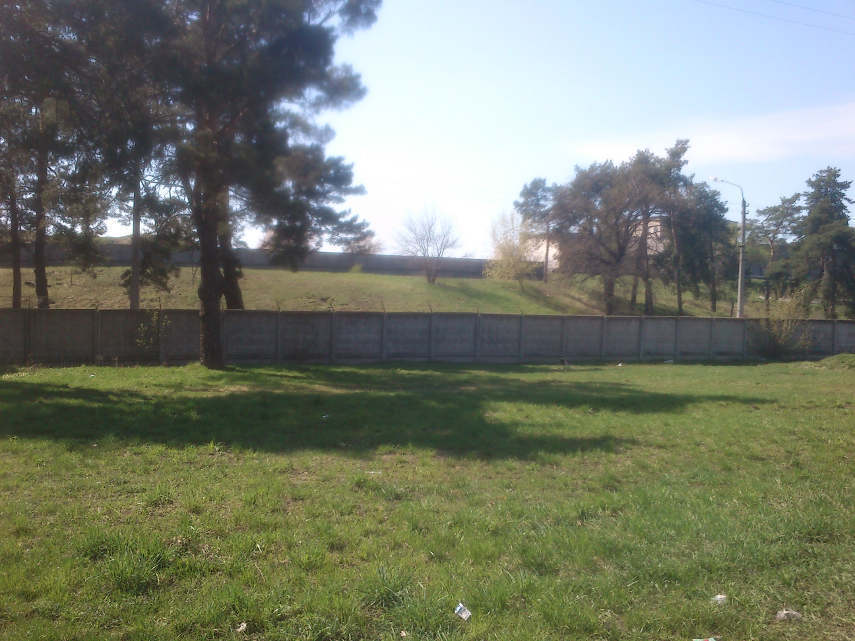
\includegraphics[width=\textwidth]{chast-gorodki/lysaya/levlys01.jpg}

\textit{Деснянская водопроводная станция.}
\end{center}
\vspace*{\fill}
Строительство жилых кварталов, проложение железной дороги (для этого на ряде участков возвели насыпи) исказили высоты местности, поэтому с точностью можно говорить только о самых очевидных, больших участках Лысой горы, лежащих в окрестностях авторынка на бульваре Перова.

Всю местность я заснял в конце лета 2017 года на видео, смотрите серию «Планеты Киева» под названием «Курганы Воскресенки».

\newpage

Северная часть Лысой горы – холм к востоку от озера Радунки – обозначена как «Песч. холм» на карте лоций 1914 года:

\vspace*{\fill}
\begin{center}
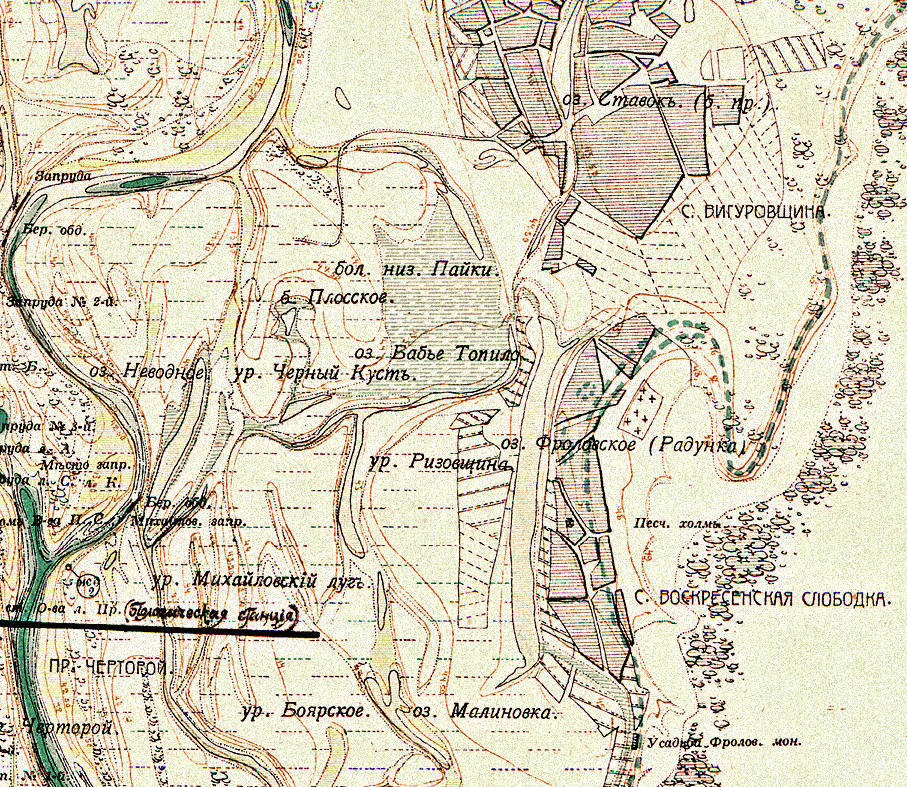
\includegraphics[width=\textwidth]{chast-gorodki/lysaya/s_1914-map.jpg}
\end{center}
\vspace*{\fill}

Вот озеро «Фроловское (Радунка)», восточнее от него село Воскресенская слободка, еще восточнее – этот песчаный холм, и к северу – кладбище. Близ верхушки сего огромного холма – а верхушка сказано сильно, она занимает приличную площадь – напротив авторынка, раньше стоял кинотеатр «Аврора». Его разрешили снести в 2004, снесли позже, теперь там торговый центр.

На самую высшую точку Лысой горы можно посмотреть возле школы номер 180 (Перова, 21-А) – там рядом впрочем есть еще одна школа, интернат, не перепутайте. Далее фотографии 2014 года, это я снимаю 180-ю школу с севера.

\newpage
\vspace*{\fill}
\begin{center}
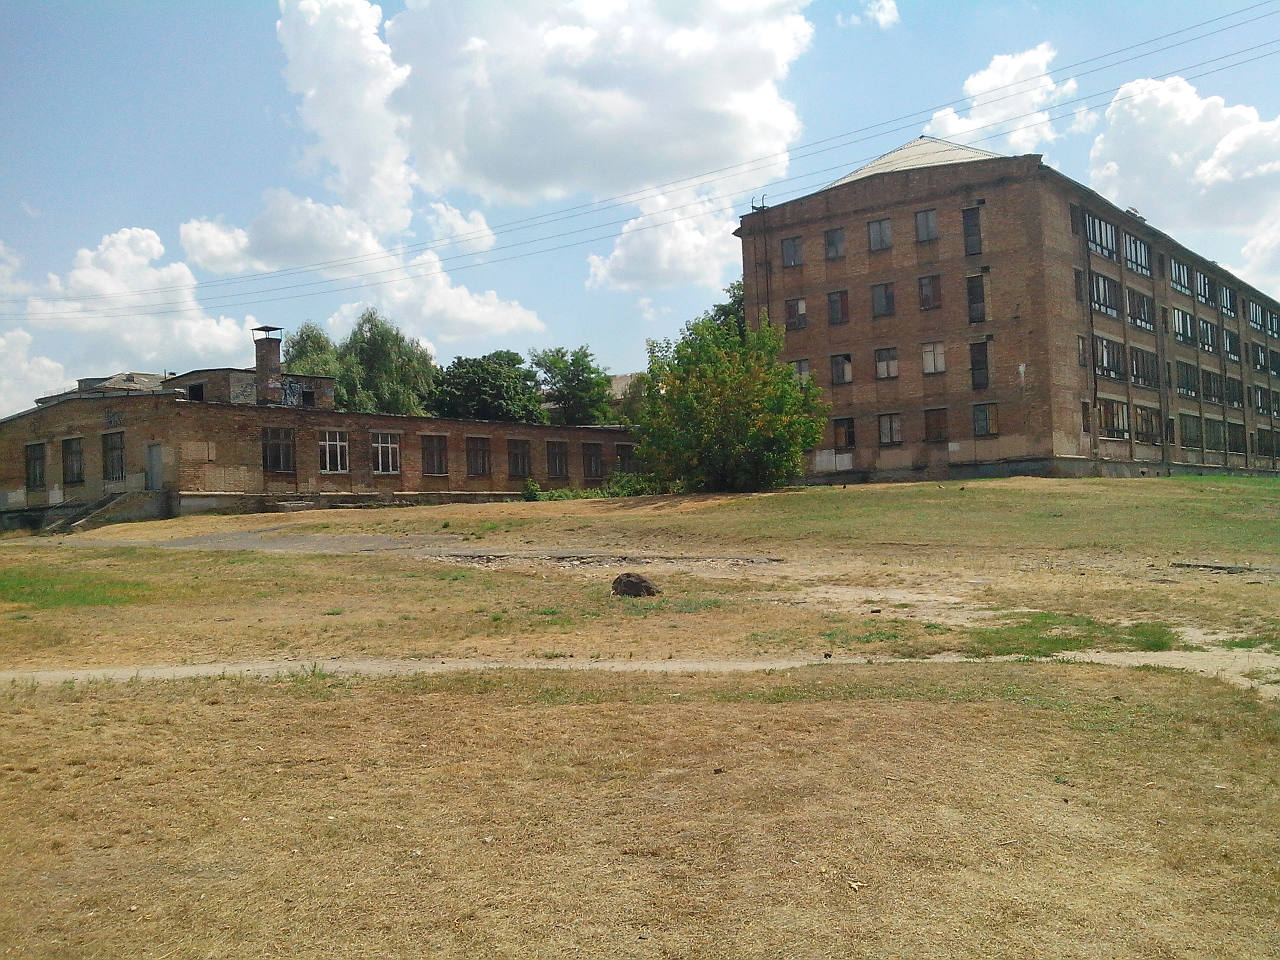
\includegraphics[width=\textwidth]{chast-gorodki/lysaya/s_IMG_20140806_124634.jpg}
\end{center}

\begin{center}
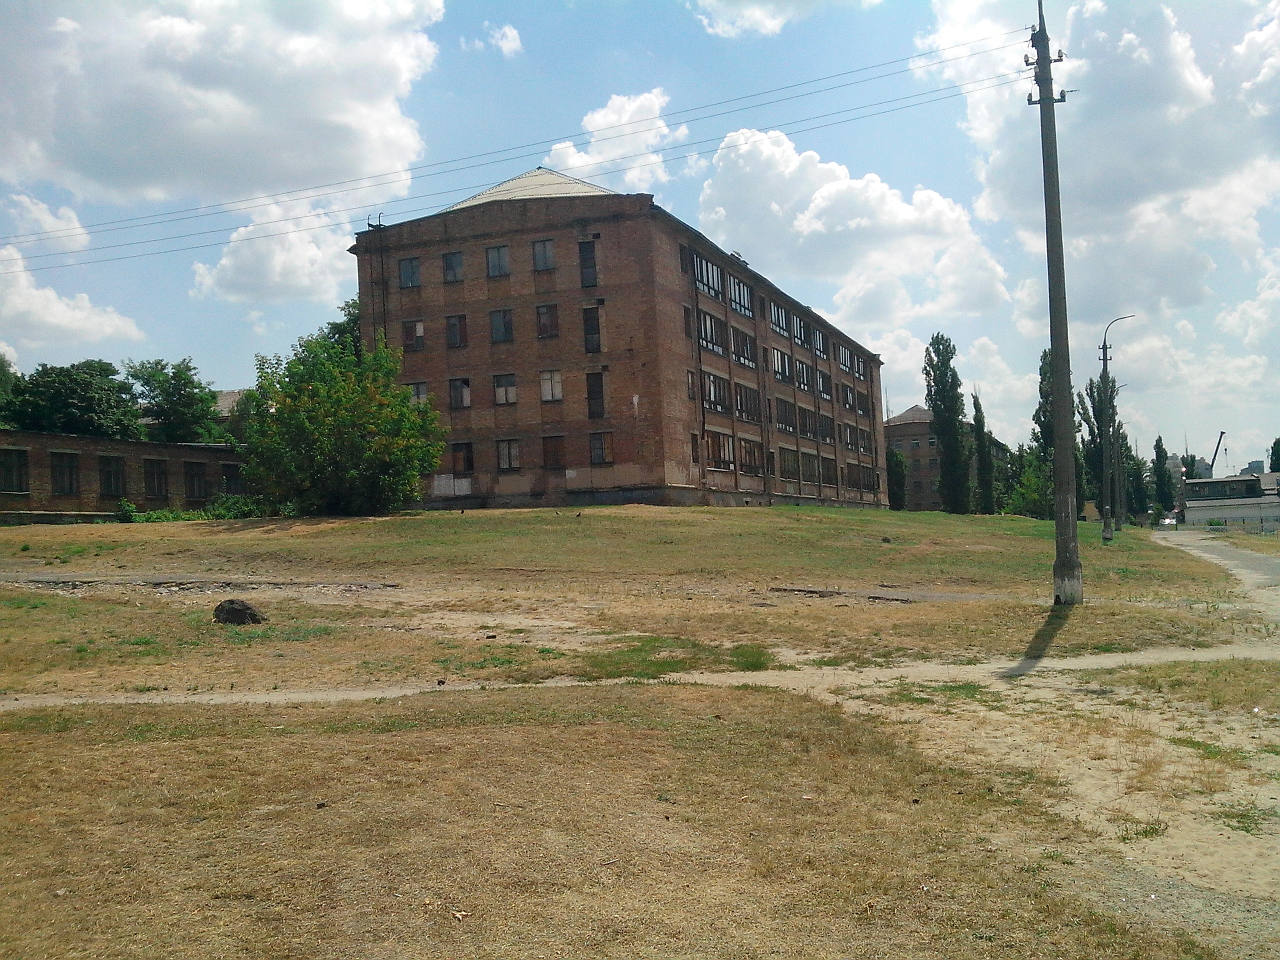
\includegraphics[width=\textwidth]{chast-gorodki/lysaya/s_IMG_20140806_124639.jpg}
\end{center}
\vspace*{\fill}
\newpage

А если выбраться оттуда назад на Перова, то дальше бульвар на север – ощутимый спуск. 

Спросите современных жителей Воскресенки и Радужного – а где здесь Лысая гора – они удивятся и скажут, что ничего про это не знают. 

Если с запада Лысая гора упирается в озеро Радунку, то с востока тоже была ограничена водоемом, хотя эта сторона более пологая. От сего, как полагаю, некогда цельного русла, ныне осталась ложбина на месте болота Куликова – вдоль улицы Крайней, затем продолжаясь на юго-запад мимо улицы Петра Запорожца, пересекая проспект Алишера Навои и по месту современного длинного пруда в парке Победы.

Таким образом жилмассивы Воскресенка и Радужный, в некотором прошлом, располагались на большом острове меж двух русел. Издавна местность если не хорошо защищенная водными преградами, то по крайней мере пригодная для жилья, в отличие от болотистых окрестностей.

Всегда ли тут были одни песчаные горбы?